\documentclass[11pt,a4paper]{article}
\usepackage[left=2cm,text={17cm,25cm},top=2cm]{geometry}
\usepackage[T1]{fontenc}
\usepackage[czech]{babel}
\usepackage[utf8]{inputenc}
\usepackage{url}
\usepackage{graphicx}
\usepackage{pdfpages}
\usepackage{algorithmicx}
\usepackage{amsmath}
\usepackage{listings}
\graphicspath{ {img/} }

\begin{document}

\begin{center}
	\LARGE{Kryptografie -- dokumentace k projektu 1}\\
	\large{Vysoké učení technické v Brně}
	\vspace{0.2cm}

	Petr Stehlík <xstehl14@stud.fit.vutbr.cz>     \today

\end{center}

\section{Zadání}

Cílem projektu bylo zjistit tajemství z několika souborů, které jsou šifrovány neznámou synchronní proudovou šifrou.


\section{Získání klíče manuální metodou}

V obdržených souborech se nachází dvojice souborů \texttt{bis.txt} a \texttt{bis.txt.enc}, kde první z nich je
nezašifrovaný textový soubor (plaintext) a druhý je šifrovaný zatím neznámou synchronní šifrou (ciphertext).

\subsection{Získání keystream}

Po aplikovaní binární operace \texttt{XOR} na soubory \texttt{bis.txt} a \texttt{bis.txt.enc} jsme schopni získat
prvních 512~B keystreamu, díky tomu, že platí vztah:

\begin{center}
    \textit{ciphertext = plaintext \texttt{XOR} keystream}
\end{center}

Kde po úpravě dostaneme:

\begin{center}
    \textit{keystream = plaintext \texttt{XOR} ciphertext}
\end{center}


\subsection{Dešifrování \texttt{super\_cipher.py.enc}}

S pomocí získáného keystreamu jsme schopni dešifrovat část zašifrovaného souboru \texttt{super\_cipher.py.enc}
(prvních 512 B) tím, že na ciphertext a keystream aplikujeme opět operaci \texttt{XOR}.

Tato operace odkryje globální proměnné a funkci \texttt{step}.
\begin{lstlisting}[language=Python,caption={Část dešifrovaného \texttt{super\_cipher.py}}]
SUB = [0, 1, 1, 0, 1, 0, 1, 0]
N_B = 32
N = 8 * N_B

# Next keystream
def step(x):
  x = (x & 1) << N+1 | x << 1 | x >> N-1
  y = 0
  for i in range(N):
    y |= SUB[(x >> i) & 7] << i
  return y

\end{lstlisting}

\subsection{Analýza \texttt{super\_cipher.py}}
Funkce step přijímá klíč $x$ o délce \texttt{N} bitů, tento klíč rozšíří o další 2 bity, původní klíč posune o
1 bit směrem k MSB a původní MSB se zduplikuje na LSB. Tím vznikne $x'$, které je následně použito pro vygenerování
keystreamu $y$. Pro generování $y$ je použito pole \texttt{SUB} a 3 bitů z $x'$, které jsou použity pro indexování v
poli \texttt{SUB}, ze kterého se získá bit, který je uložen do $y$. Takto vygenerovaný keystream je poté vrácen.

Všechny operace ve funkci \texttt{step} jsou reverzovatelné a tudíž bude možné získat počáteční klíč.

\subsection{Dešifrování dalších souborů}

Pro dešifrování souborů delších než 512 B je potřeba keystream vygenerovat ve stejné velikosti jako je daný plaintext.
Po experimentování s různými způsoby bylo odhaleno, že pokračování keystreamu lze vytvořit aplikováním funkce
\texttt{step} na první blok keystreamu velikosti \texttt{N} bitů získáného v předchozích krocích.

Díky tomuto postupu bylo možné úspěšně dešifrovat kompletní obsah souborů \texttt{super\_cipher.py.enc} a
\texttt{hint.gif.enc}. Po dešifrovaní Python skriptu a obrázku vidíme jak je šifra aplikovaná na celý plaintext a jak
je použitý klíč.


\begin{figure}[h]
    \center
    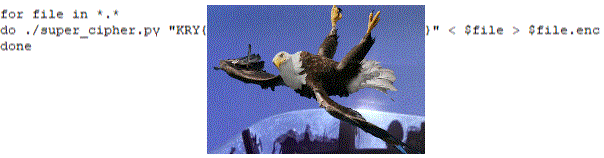
\includegraphics[width=0.75\linewidth]{hint}
    \caption{Dešifrovaný soubor \texttt{hint.gif}}
\end{figure}

\subsection{Získání tajemství}

Pro získání původního klíče je nutné reverzovat funkci \texttt{step}. Pro určení bitu na dané pozici musíme určit 3 bity
původního keystreamu. To celkově vede ke 4 možnostem jak daný bit mohl být určený indexací do pole \texttt{SUB}. Nicméně
každý bit klíče sdílí 2 bity původního keystreamu se svými okolními bity. To značně usnadňuje vyhledání správného bitu.

Reverzování algoritmu ve funkci \texttt{step} vyzkouší všechny možné kombinace, které k danému bitu mohly vést a pokud
první dva a poslední dva bity jsou stejné, jde o kandidáta na získání původního klíče, kde k existujícím kandidátům
přidáme danou trojici bitů, které indexovaly zkoušený bit.

Jakmile máme všechny možné kandidáty využijeme znova této vlastnosti a najdeme klíč, který má dva LSB a dva MSB stejné.

Na tento klíč následně aplikujeme invertované operace pro modifikaci $x$ z funkce \texttt{step} a tím získáváme námi
hledaný klíč.

Je zde možnost nalezení kolizního klíče, která je ale v případě 32 B klíče velmi malá a klíč získaný z obdržených
souborů není kolizní, proto tuto situaci dešifrovací skript nezohledňuje.

\section{Ovládání \texttt{solution.py}}
Program \texttt{solution.py} disponuje přepínačem \texttt{-d}, který dešifruje soubory ve složce \texttt{in/} a uloží je
do této složky.

\section{Závěr}
Manuální řešení získávání počatečního klíče bylo úspěšně implementováno a bylo získáno tajemství, které je pro
poskytnuté soubory následující: \texttt{KRY\{xstehl14-51f610e23c2b4e9\}}.

Řešení pomocí SAT nebylo implementováno.

\end{document}

